\section{Tritiated Methane Removal}
\label{sec:RD}

CH$_3$T removal efficiency of zirconium getters had previously been studied at the University of Maryland.  It was found that ..... [ATTILA'S PAPER]. Additionally, a table top gaseous xenon system was developed at the University of Maryland to examine the effects of residuals contamination after injecting CH$_3$T.  It was found that a SAES MC1-905F methane purifier placed in series immediately after the CH$_3$T source bottle was required to prevent tritium from non-methane species from contaminating the plumbing. Using the result of these two studies, a small scale tritiated methane injection system was integrated into a liquid xenon system at the University of Maryland.  After cumulatively injecting over 68,000 Bq of observed CH$_3$T we were able to achieve purification efficiencies ranging from 99.983\% - 100\%, with an average purification efficiency of 99.999\% in our liquid experiments, where we define our purification efficiency to be

\begin{center}
Purification Efficiency $= 1 - \frac{A - B}{I - B},$
\end{center}

\noindent
where $A$ is the background event rate after injecting CH$_3$T, $B$ is the background event rate prior to injecting CH$_3$T, and $I$ is the injected CH$_3$T activity as observed by out PMTs.  

\begin{figure}[h!]\centering
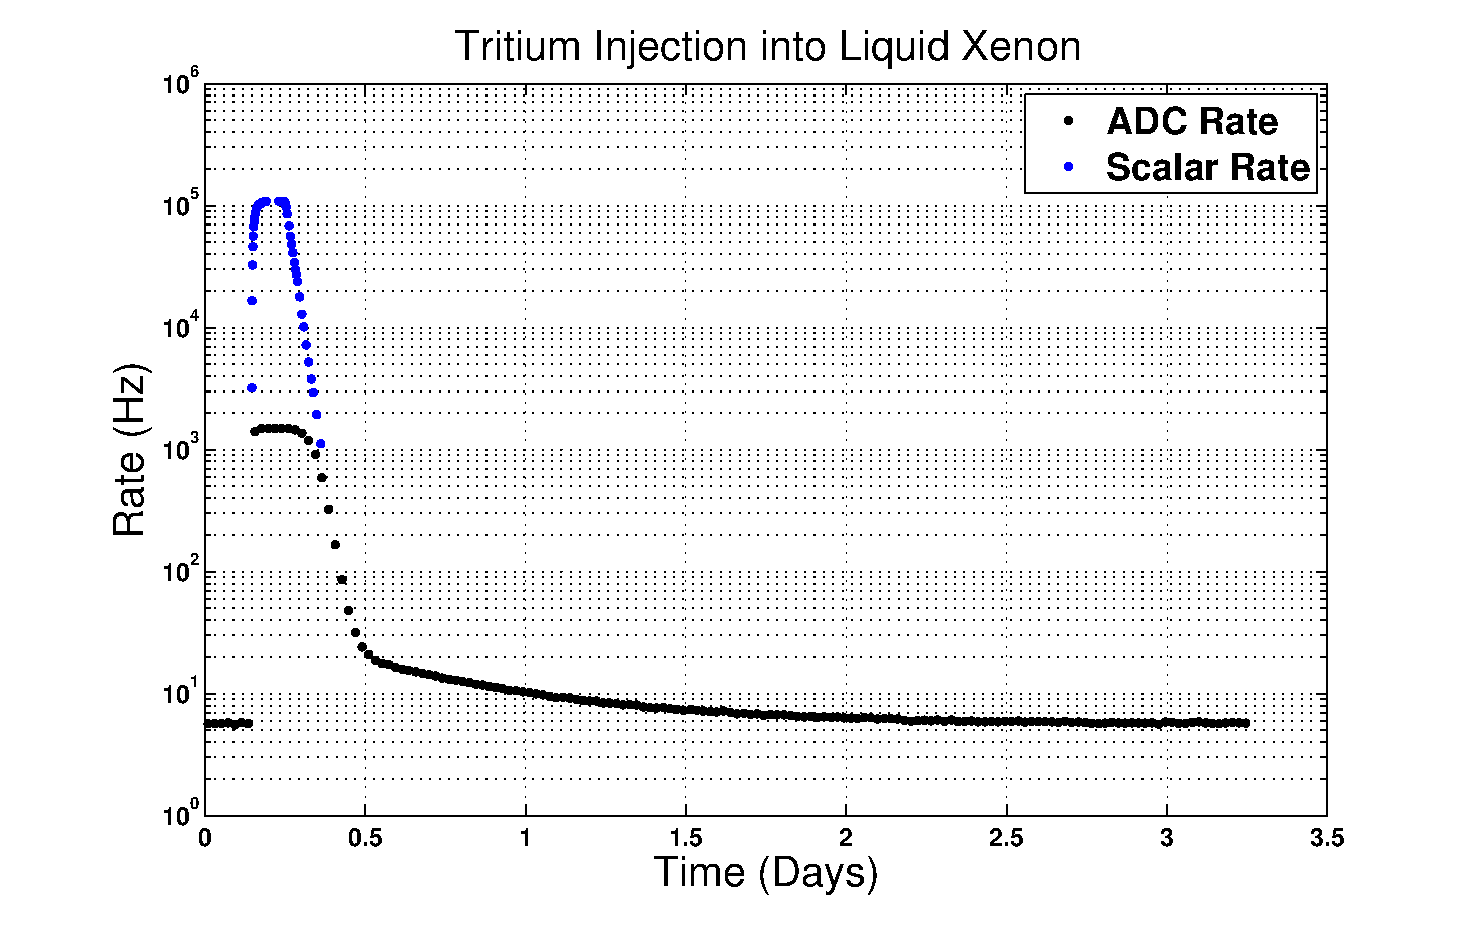
\includegraphics[width=100mm]{TimeHisto_Analog2.eps}
\caption{A time histogram of the event rate during a tritium injection into our small scale detector. The event rate greatly exceeded the limits of our ADC (black data points), so a analog scalar was used to count the true event rate (blue data points). }
\label{fig:Density}
\end{figure}


The liquid system was also used to study the effect of out gassing from plastics on the residual background rate after a CH$_3$T injection.  We found that the addition of plastic curtains around our PMTs does not impair our ability to remove CH$_3$T at $>$ 99.998\% levels. 